% 2013 全国卷Ⅰ理科第 17 题：直角三角形 ABC 与内点 P 的连线。
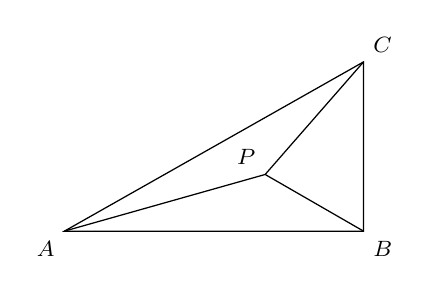
\begin{tikzpicture}[font=\footnotesize, line width=0.45pt]
  \coordinate (A) at (0,0); \coordinate (B) at (3.8,0); \coordinate (C) at (3.8,2.15);
  \coordinate (P) at (2.55,0.72);
  \draw (A)--(B)--(C)--cycle;
  \draw (P)--(A) (P)--(B) (P)--(C);
  \node[below left] at (A) {$A$}; \node[below right] at (B) {$B$};
  \node[above right] at (C) {$C$}; \node[above left] at (P) {$P$};
\end{tikzpicture}
